% Chapter Template

\newcommand{\reals}[1]{\mathbb{R}^{#1}}

\chapter{Proposals} % Main chapter title
\label{Chapter3}

As we have already seen in Chapter \ref{Chapter2}, LUSI introduces a new data-driven learning
paradigm which aims to find better approximations of the conditional probability function using
statistical invariants. However, these invariants are often problem dependent and choosing the
appropriate ones is not an easy task, as there are many possible ones and some of them are not
straightforward to come up with.

Thus, our main goal with this work is to create a series of new invariants which we expect to be of
general use, as well as automatizing the selection process of the invariants that should be considered
for a given problem and extending the LUSI paradigm to multiclass problems\footnote{Even though in the
original paper the authors state that the method can be applied to multiclass problems, they do not go
into too much detail of how this is done.}.

In this chapter we are going to present our proposals, which are a two new invariants based on randomness
which aim to be more general than the original ones and an extension of the LUSI paradigm to multiclass problems
using Error Correcting Output Codes (ECOC).

\section{Random invariants}

Our first proposal is a series of random invariants, which are invariants that have some sort of random
process inside of them but that aim to preserve some sort of statistical information of the data. This way,
we aim to greatly reduce the amount of necessary prior knowledge of the problem when choosing which invariants
to use, treating it just like any other hyperparameter of a machine learning model. In this work, we propose
an invariant based on random projections as well as another one based on random hyperplanes.

\subsection{Random projections}

Random projections have been frequently used in the machine learning field to perform dimensionality reduction
in a faster and computationally less expensive way than other techniques (i.e., PCA) as studied in 
\cite{Dasgupta2000} and \cite{BinghamManila2001}.

In our case, the random projection invariant offers a glimpse of the data from a different viewpoint
and compresses the data into a single dimension as if it was viewed from that particular point.
Intuitively, this can be observed in figure \ref{fig:random_projections_example}.

More formally speaking, consider a data point $x \in \reals{d}$ and a projection vector
$p \sim \mathcal{N}(\mu, \Sigma)$, where the multivariate normal distribution has mean $\mu \in \reals{d}$
and covariance matrix $\Sigma \in \reals{d \times d}$. We can define the random projection invariant as follows:

\begin{equation}
    \label{eq:random_projection_invariant}
    \psi_{r.p.}(x) = x p
\end{equation}

As we can see in expression \eqref{eq:random_projection_invariant}, we are computing the dot product between
the data point and the projection vector. When this invariant is used in expression \ref{eq:invariant_approximation}
it will try to preserve the centroid of the positive class in the new projected space. Hence, it is a variation
of the first order invariant. When using multiple random projections as invariants, we expect that the centroid
of the positive class is preserved across different views of the data.

\begin{figure}[h]
    \centering
    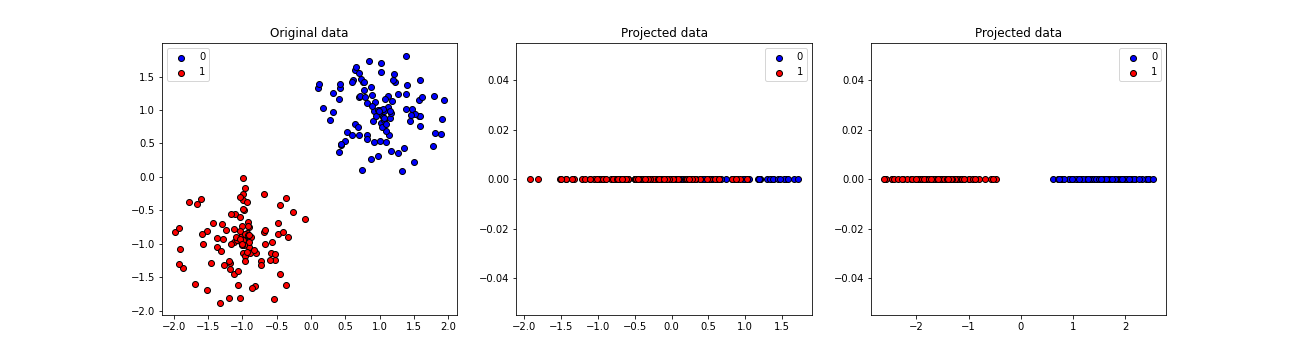
\includegraphics[width=\textwidth]{thesis/Figures/random_projections_example}
    \caption{Example of a dataset and two random projections of it. In the first projection, we can see
    that the points from the red and blue classes are almost totally overlapped, whereas in the second projection
    they are completely separable.}
    \label{fig:random_projections_example}
\end{figure}

\subsection{Random hyperplanes}

The second invariant that we propose is the random hyperplane. With it, we aim to create two partitions of
the original data: the samples that are on the right side of the hyperplane and the ones on the left, which
we will consider as the positive and the negative samples, respectively. Opposite to the previous invariant, which
produced a real value when applied to a point $x$, this one produces a discrete value $\set{0, 1}$ based on the
relative position of the point with respect to the normal vector of the hyperplane.
Figure \ref{fig:random_hyperplanes_example} shows an example of how this invariant works when applied to
an example dataset.

Formalizing the previous explanation, consider an arbitrary point from the sample $x_c$. Let
$n \sim \mathcal{N}(\mu, \Sigma)$ be the normal vector of the hyperplane that contains $x_c$, where the
multivariate normal distribution has mean $\mu \in \reals{d}$ and covariance matrix $\Sigma \in \reals{d \times d}$.
We can define the random hyperplane invariant as

\begin{equation}
    \label{eq:random_hyperplane_invariant}
    \psi_{r.h.}(x) =
    \begin{cases}
        1 & \text{if $(x - x_c)n \geq 0$ }\\
        0 & \text{otherwise}
    \end{cases}
\end{equation}

Considering the previous expression, we can clearly see that this invariant will yield a vector of zeroes
and ones when applied to the data sample. If we also take into account expression \eqref{eq:invariant_approximation},
we can deduce that this invariant will try to preserve the proportion of positive samples that fall on the right
side of the hyperplane. Consequently, we can see that this is a variation of the zeroth order invariant.
The main difference is that we are now trying to preserve the proportion of positive elements in a subspace
of the original space (the subspace formed by the samples that are on the same side as the normal vector of the
hyperplane), instead of trying to preserve it in the whole space.

\begin{figure}[h]
    \centering
    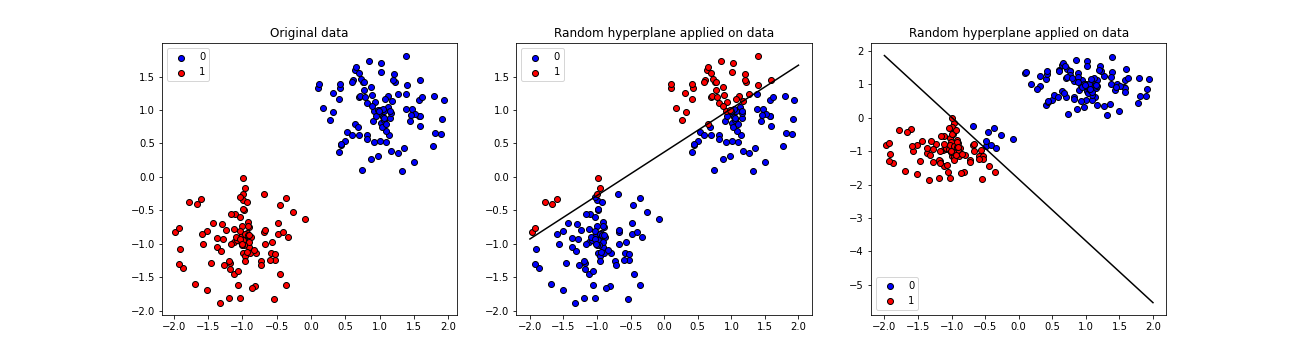
\includegraphics[width=\textwidth]{thesis/Figures/random_hyperplanes_example.png}
    \caption{Example of the hyperplanes invariant. In the left image, we can see the original data. In
    the middle and right images we can see two hyperplanes that divide the data in elements which are
    on the right and the left of the hyperplane, labeled as 1 and 0 respectively. Note that these
    new labels do not necessarily match the original ones.}
    \label{fig:random_hyperplanes_example}
\end{figure}

\section{Extending the LUSI paradigm to multiclass problems}

